\documentclass[11pt]{article}


\usepackage[utf8]{inputenc}
\usepackage{tikz}
\usepackage{tikz-3dplot}
\usepackage{tikz-cd}
\usepackage{xcolor}
\usepackage{proof}
\usepackage {alltt}

\usepackage{graphicx} % Allows including images
\usepackage{booktabs} % Allows the use of \toprule, \midrule and \bottomrule in tables
\usepackage{listings}
\usepackage[export]{adjustbox}
\usepackage{verbatim}
\tikzset
  {cross/.style={cross out, draw=black, minimum size=2*(#1-\pgflinewidth), inner sep=0pt, outer sep=0pt},cross/.default={1pt}}

\usetikzlibrary{decorations.markings}
\usepackage{amsmath }
\usepackage{framed}
\usepackage{proof}
\usepackage{enumerate,xspace,stmaryrd}
\usepackage{amsmath,amssymb,latexsym}
\usepackage{textcomp,xspace}
\usepackage[top=2cm, bottom=2.5cm, right=2.5cm, left=2.5cm]{geometry}\usepackage{latexsym}  %For plain TeX symbols, such as \Box used in \qed
\usepackage{euscript}  %%Euler Script font
\usepackage {mdframed}
\usepackage{ifpdf}
\usepackage {alltt}
\renewcommand{\ttdefault}{txtt}
\ifpdf
  \usepackage{epstopdf}
\fi 
\usepackage{etoolbox}
\BeforeBeginEnvironment{tabular}{\begin{center}\small}
\AfterEndEnvironment{tabular}{\end{center}}

\newcommand{\A}{{\ensuremath{\mathbb A}}\xspace}
\newcommand{\B}{{\ensuremath{\mathbb B}}\xspace}
\newcommand{\C}{{\ensuremath{\mathbb C}}\xspace}
\newcommand{\D}{{\ensuremath{\mathbb D}}\xspace}
\newcommand{\F}{{\ensuremath{\mathbb F}}\xspace}
\newcommand{\G}{{\ensuremath{\mathbb G}}\xspace}
\newcommand{\R}{{\ensuremath{\mathbb R}}\xspace}

\newcommand{\rst}[1]{\overline{#1}\,}
\newcommand{\Sets}{{\ensuremath{\sf Sets}}\xspace}
\newcommand{\Cat}{{\ensuremath{\sf Cat}}\xspace}
\newcommand{\llab}[1]{\tiny{\texttt{(+)~~~}}
                      \small{$#1$}
                      \tiny{\texttt{~~~(-)}}
                     }
\newcommand{\plab}[1]{\tiny{\texttt{(+)~~~}}
                      \small{$#1$}
                     }



\newcommand{\proc}[2] {\small{\sf{$#1$}}\\~~\\ \tiny{{#2}}}

\input xy
\xyoption{all}
\xyoption{2cell}
\UseAllTwocells

\title{Concurrent MPL}

\bibliographystyle{plain}

%%%%%%%%% macros defined %%%%%%%%%%%%%%%%%%%%%%%%%%%%%%%%%%%%%%%%%

\newcommand{\X}{{\ensuremath{\mathbb X}}\xspace}
\newcommand{\Y}{{\ensuremath{\mathbb Y}}\xspace}
\newcommand{\Z}{{\ensuremath{\mathbb Z}}\xspace}

\newcommand{\<}{\langle}
\renewcommand{\>}{\rangle}
\newcommand{\lollipop}{\ensuremath{-\!\!\circ}}

\newcommand{\op}{\ensuremath{^{\textnormal{op}}}}
\renewcommand{\hat}{\widehat}
\renewcommand{\b}{\bullet}
\renewcommand{\c}{\circ}
\newcommand{\ox}{\otimes}         
\newcommand{\x}{\times}     
\newcommand{\fold}[1]{\ensuremath{\left\{\!\!\!\;\left| #1 \right|\!\!\!\;\right\} }}  
\newcommand{\unfold}[1]{\ensuremath{\left(\!\!\!\;\left| #1 \right|\!\!\!\;\right) }}  
\def\endproof{~\hfill$\Box$\vskip 10pt}

\newtheorem{theorem}{Theorem}[section]    
\newtheorem{corollary}[theorem]{Corollary}   
\newtheorem{lemma}[theorem]{Lemma}   
\newtheorem{remark}[theorem]{Remark}   
\newtheorem{example}[theorem]{Example}   
\newtheorem{proposition}[theorem]{Proposition}
\newtheorem{definition}[theorem]{Definition}

\newcommand{\proof}{\noindent{\sc Proof:}\xspace}

\def\monus{\buildrel\textstyle.\over
    {\hbox{\vrule height.55ex width0pt
        \smash{\hbox{\mathsurround=0pt$-$}}}}}
\def\xybox#1#2{\save [].[#2]!C="xb#1"*[F.]\frm{}\restore}


\begin{document}
\maketitle

\section {Concurrent MPL constructs}
Concurrent MPL constructs are the constructs using which concurrent MPL programs are written. In this chapter, various concurrent MPL constructs are discussed.

\section {Introduction}
Concurrent MPL constructs are {\sf plug}, {\sf id}, {\sf hput-hcase}, {\sf get-put}, {\sf split-fork} and {\sf close-halt}. A few noticeable observations about concurrent MPL constructs are below:
\begin{itemize}
  \item MPL constructs with the exception of {\sf run} contruct perform an action on a channel. In MPL concurrency is modeled using {\em message passing} between processes and channels are the conduit through which the messages are exchanged. So, it is only logical that most constructs deal with channel.
  \item Most concurrent MPL constructs come in pair, i.e {\sf get-put}, {\sf hput-hcase}, {\sf split-fork} and {\sf halt-close}. {\sf id}, {\sf run} and {\sf plug} are standalone constructs. The constructs of the pair are dual to each other.
  This is intuitive because in message passing view of concurrency for someone to respond to an action, someone else should drive that action on the opposite end of the channel and viveversa. Thus one of the constructs of in a pair is a driver construct and the other is a reaction construct. For example, for a process to receive a value on a channel, some other process should have put a value on the channel.
\end{itemize}

A brief description of the constructs are as below:

\begin{table}[!h]
\begin{center}
    \begin{tabular}{|l||l|}
    \hline 
        {\sf run} & calls a process \\ \hline 
        {\sf id}  & equates two channels \\ \hline 
        {\sf plug} & connects two processes by a channel \\ \hline  
        {\sf get} & gets a value on a channel \\ \hline 
        {\sf put} & puts a value on a channel \\ \hline 
        {\sf hput} & puts a handle on a channel \\ \hline 
        {\sf hcase} & cases on the handles obtained on channel \\ \hline 
        {\sf split} & splits a channel into two channels \\ \hline 
        {\sf fork} & forks two new processes \\ \hline 
        {\sf close} & closes a channel \\ \hline 
        {\sf halt} & closes a channel. Usually the last channel is halted. \\ \hline
   \end{tabular}
\caption{Machine Transitions for the SAMPL}
\label{AMPL:TranSeqTable}
\end{center}
\end{table}

In the next section, the concurrent MPL constructs are described in details.

\section{get-put}
These are the simplest MPL constructs. {\sf get} receives a value on a channel and {\sf put} puts a value on a channel. 
\begin{itemize}
  \item On an output channel, {\sf get} results in {\bf Get} protocol and {\sf put} results in {\bf Put} protocol.
  \item On an input channel, {\sf get} and {\sf put} constructs result in {\bf Put} and {\bf Get} protocols respectively.
\end{itemize}
Thus, {\sf get/put} constructs result in different protocols depending on the polarity of the channel over which they act. This is done in order to infer the same protocol for a channel from the two processes attached at the two ends of the channel.

\subsection {get-put Example}
Table \ref {fig:Conc_getput} shows an example of an MPL program that uses {\sf get-put} construct. The process connectivity diagram of an MPL program represents how different processes of the program are connected via channels. Figure \ref {Conc : getputExample} represents the process connectivity diagram for the example program in Table \ref {fig:Conc_getput}.
~~\\~~\\ 
In the program there are three processes, $\mathbf {p1}$, $\mathbf {p2}$ and $\mathbf {p3}$ apart from the main process. These processes have been represented by three circles named as $\mathbf{P_1}$, $\mathbf{P_2}$ and $\mathbf {P_3}$ respectively in the process connectivity diagram.
~~\\~~\\
Channel $\mathbf {ch2}$ is plugged between processes $\mathbf {p2}$ and $\mathbf {p3}$ and channel $\mathbf {ch1}$ is plugged between processes $\mathbf {p3}$ and $\mathbf {p1}$. These channels are drawn as solid lines joining $\mathbf {P_2}$-$\mathbf {P_3}$ and $\mathbf {P_3}$-$\mathbf {P_1}$ respectively in the process connectivity diagram. $\mathbf {ch2}$ acts as an output channel for process $\mathbf {p2}$ and an input channel for process $\mathbf {p3}$. The $\mathbf {\texttt{(+)}}$ sign on $\mathbf {ch2}$ at process $\mathbf {P_2}$'s end and $\mathbf {\texttt{(-)}}$ sign on $\mathbf {P_3}$'s end represents the polarity of channel with respect to the two processes it is plugged between.

\begin{table}[h!]
\begin{center}
\begin{tabular}{|c|} \hline
\begin{minipage}{5in}
{
\begin{alltt}


    protocol IntTerm (A) => P =
        GetInt    :: Get (A|P) => P 
        PutInt    :: Put (A|P) => P
        Close     :: TopBot    => P  


    proc p2 :: |  => IntTerm (Int),Put(Int|TopBot) =
        |  => s1,ch2 -> do 
            hput GetInt on s1
            get x on s1
            put x on ch2
            hput Close on s1
            close s1 
            halt ch2


    proc p3 :: |  Put (Int|TopBot) => Put (Int|TopBot) =
        | ch2 => ch1 -> do 
           get x on ch2
           put x on ch1 
           close ch2
           halt ch1

    proc p1 :: | Put (Int|TopBot) => IntTerm (Int) = 
         | ch1 => s2 -> do 
            get x on ch1 
            hput PutInt on s2 
            put x on s2 
            hput Close on s2 
            close s2
            halt ch1

    run => intTerm1,intTerm2 -> do 
        plug
          p2 ( | => intTerm1,ch2)  
          p3 ( | ch2 => ch1) 
          p1 ( | ch1 => intTerm2 )



\end{alltt}

} 
\end {minipage} 
\tabularnewline
\hline
\end{tabular}
\caption{Example : {\sf get-put} constructs}
\label{Conc : getputExample}
\end{center}
\end{table}


\begin{figure}[!h]
\begin{center}
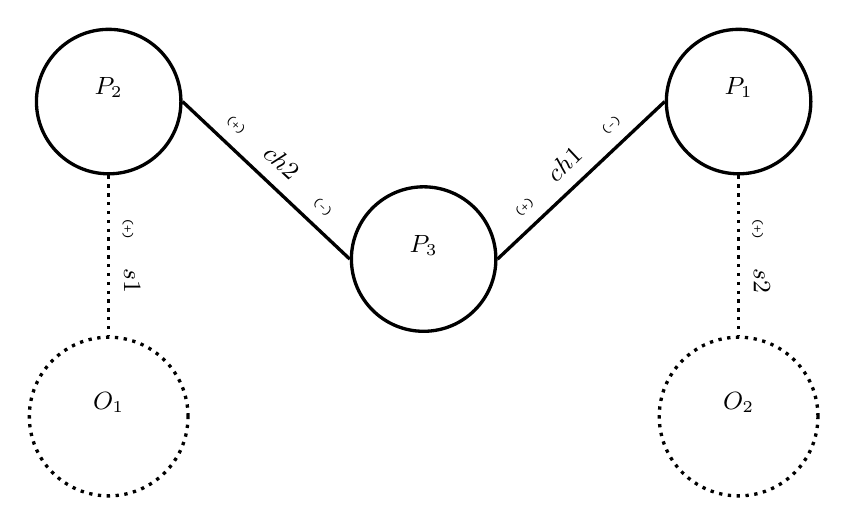
\begin{tikzpicture}[ scale = 2,
                     every node/.style={very thick},draw = black,
                   ]
 \draw (0,0)  node[circle,draw=black,text width = 1.4cm,align=center] (A) 
              {\proc{P_2}{ 
                         }
              };

 \draw (4,0)  node[circle,draw=black,text width = 1.4cm,align=center] (B)
              {\proc{P_1}{ 
                         }
              };

 \draw (4,-2) node[circle,draw = black,text width = 1.6cm,align=center,dotted] (D)
              {\proc{O_2}{}
              };

 \draw (0,-2) node[circle,draw=black,text width = 1.6cm,align=center,dotted] (E)
              {\proc{O_1}{}
              };

 \draw (2,-1) node[circle,draw=black,text width = 1.4cm,align=center] (C) 
              {\proc{P_3}{
                         }
              };

 \draw[-,draw=black,very thick] (A.east) -- (C.west) 
    node[midway,above=1pt,sloped,fill=white]   {\llab{ch2}};
 \draw[-,draw=black,very thick] (C.east) -- (B.west) 
    node[midway,above=1pt,sloped,fill=white]   {\llab{ch1}};
 \draw[-,draw=black,very thick,dotted] (B.south) -- (D.north) 
    node[midway,above=1pt,sloped,fill=white]   {\plab{s2}};
 \draw[-,draw=black,very thick,dotted] (A.south) -- (E.north) 
    node[midway,above=1pt,sloped,fill=white]   {\plab{s1}};

\end{tikzpicture}
\end {center}
\caption{{\sf get-put} Example} 
\label{fig:Conc_getput}\end{figure}
\end {document}

